\section{Resultados}\label{sec:resultados}

\subsection{Features}\label{subsec:features}

Realizamos un \textit{scatter plot} de los datos, exponemos los resultados en la figura \ref{fig:trending}.

\begin{figure}[hbtp]
  \centering
  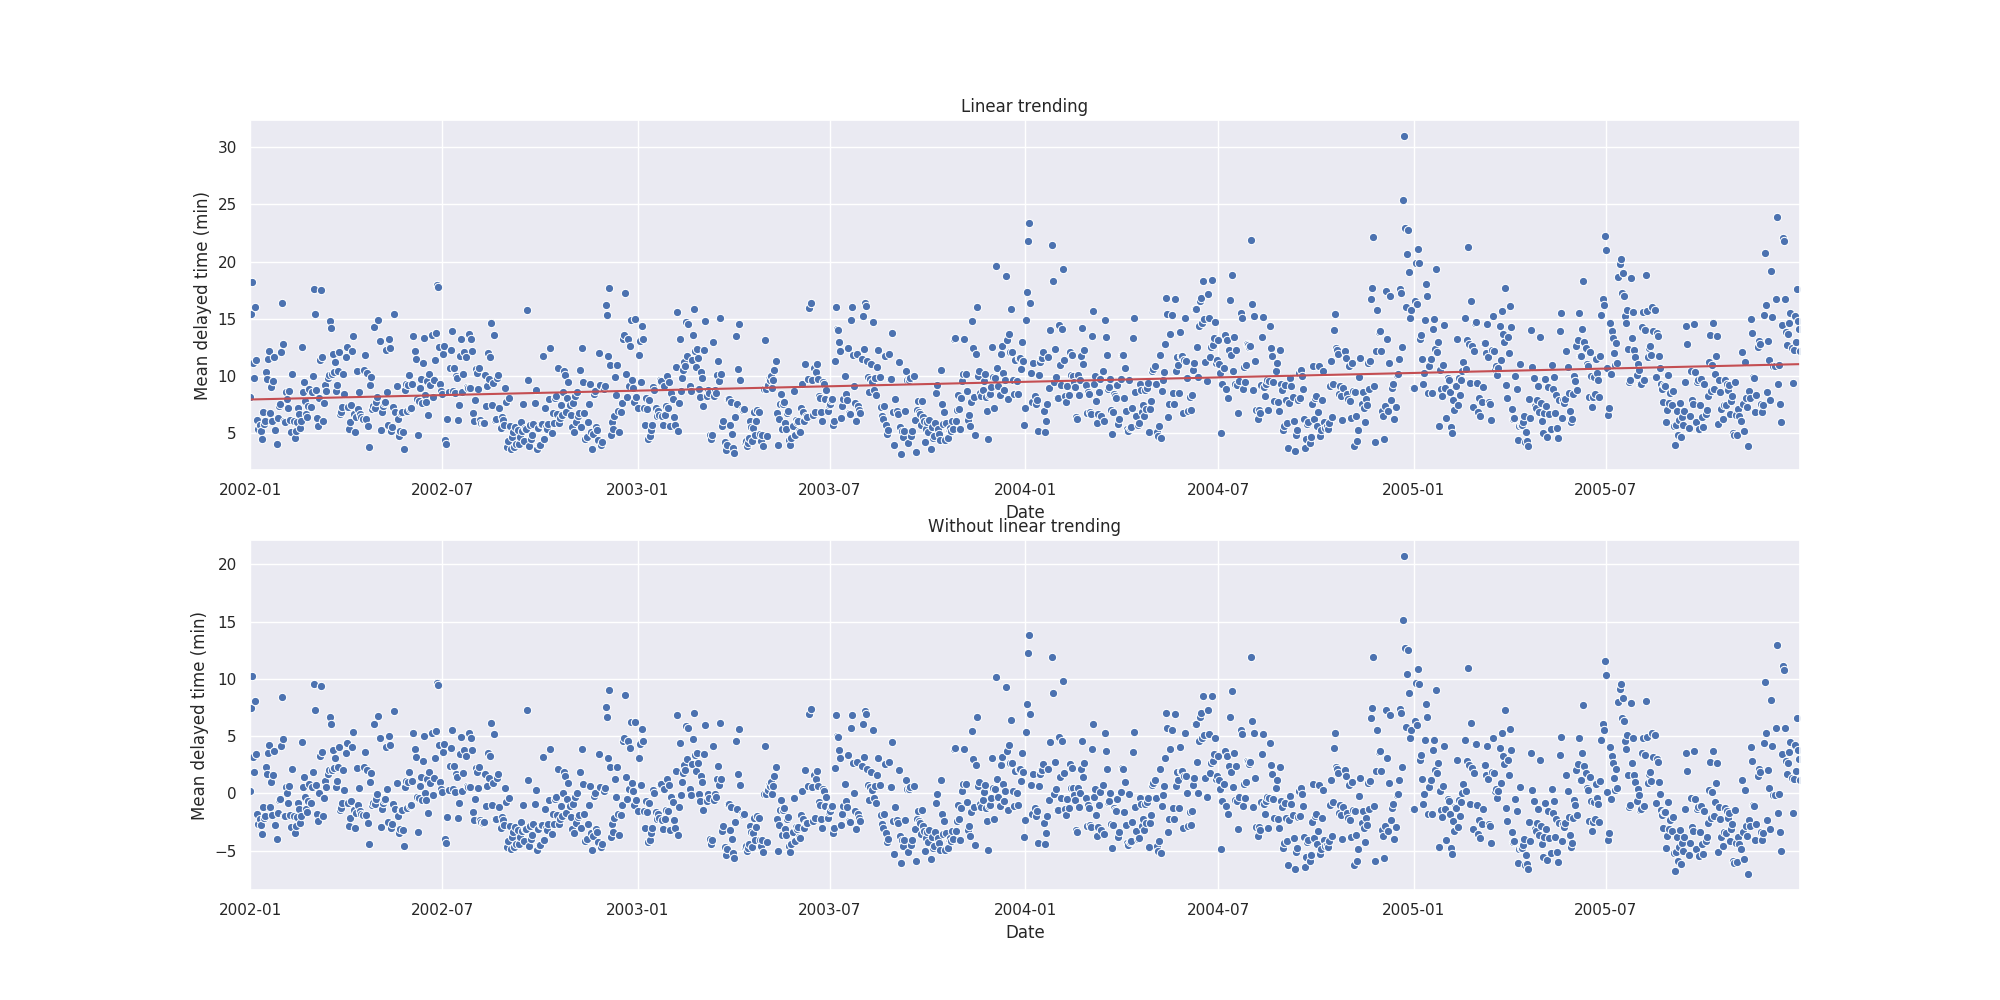
\includegraphics[width=\textwidth]{plots/linear_trending.png}
  \caption{Detrending de los datos}
  \label{fig:trending}
\end{figure}

Realizamos un ajuste lineal de los datos, los que nos da un nuevo dataset con media cero (proceso conocido
como \textit{detrending}).

Luego, realizamos gr\'aficos que nos muestren c\'omo se comportan los retrasos dentro de los meses de un a\~no, los
d\'ias de un mes y los d\'ias de una semana. Exponemos los datos en las figuras \ref{fig:within_year}, \ref{fig:within_month}
y \ref{fig:within_week}.

\begin{figure}[hbtp]
  \centering
  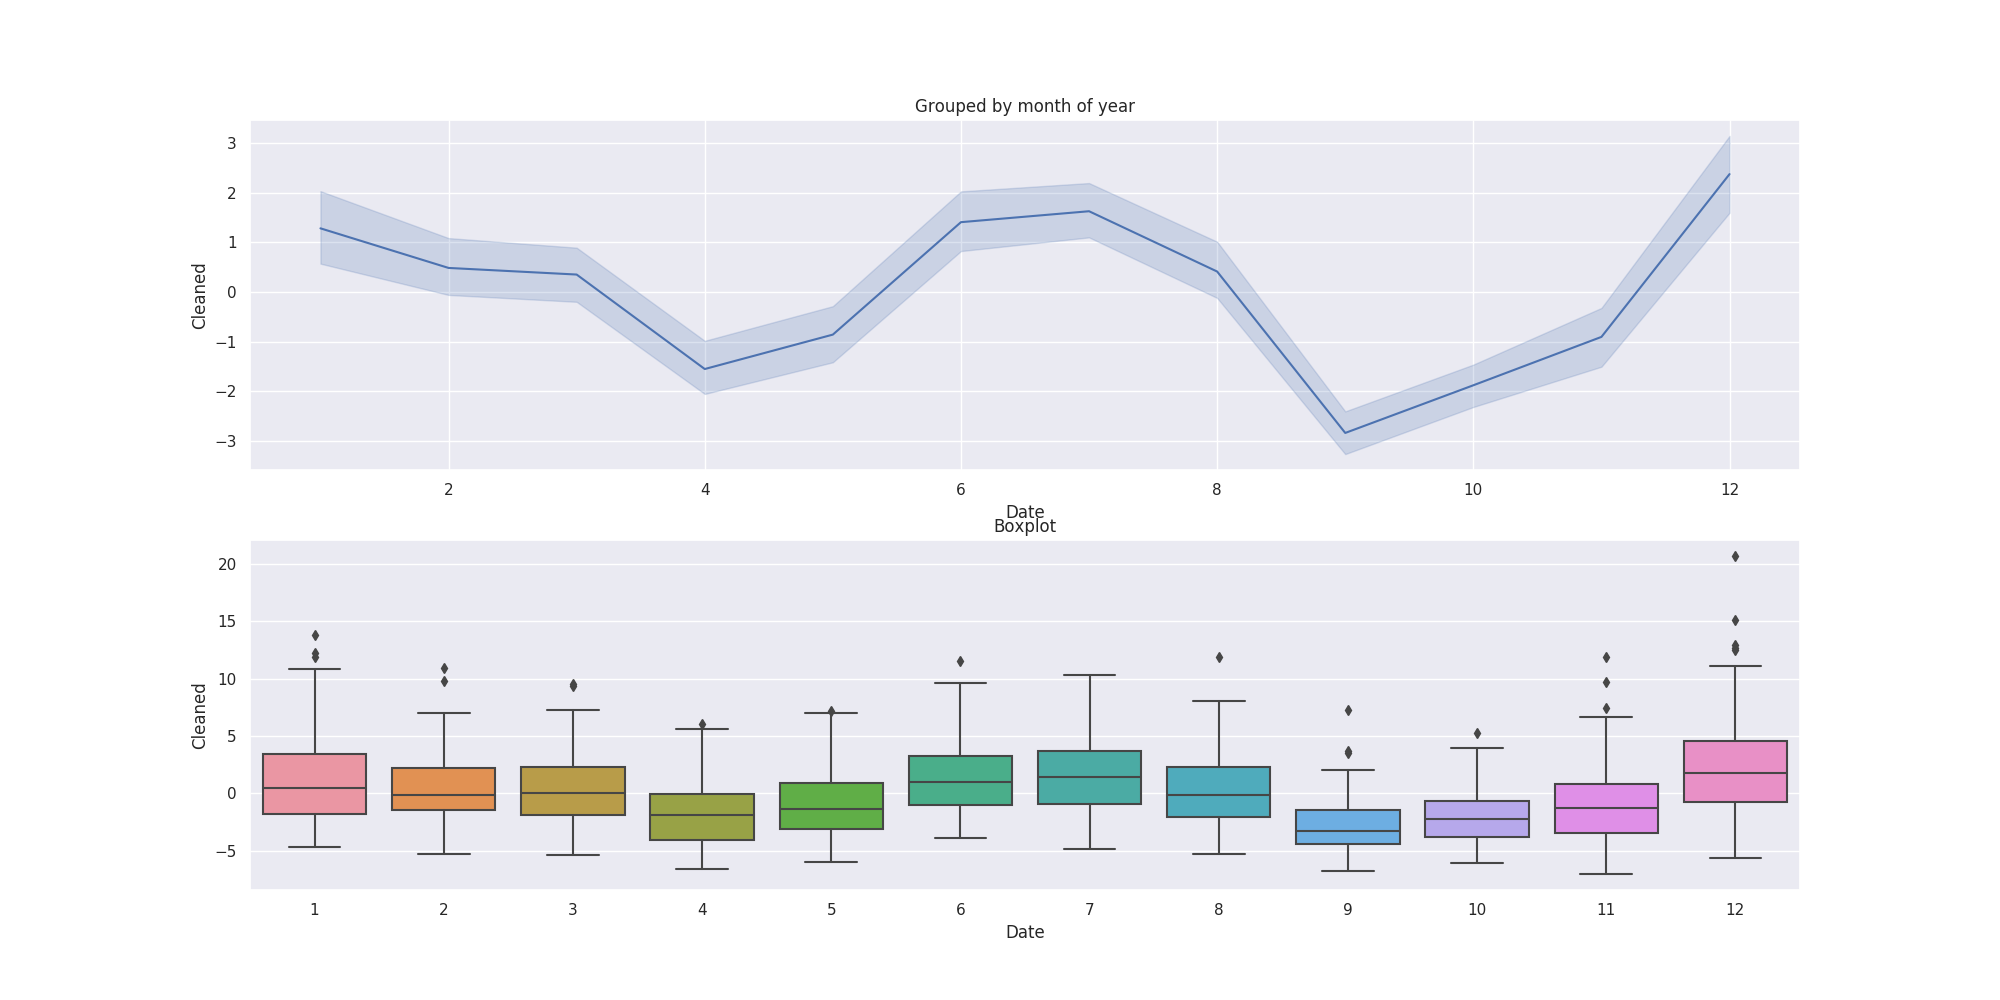
\includegraphics[width=0.7\textwidth]{plots/within_year.png}
  \caption{Retraso medio por mes}
  \label{fig:within_year}
\end{figure}

\begin{figure}[hbtp]
  \centering
  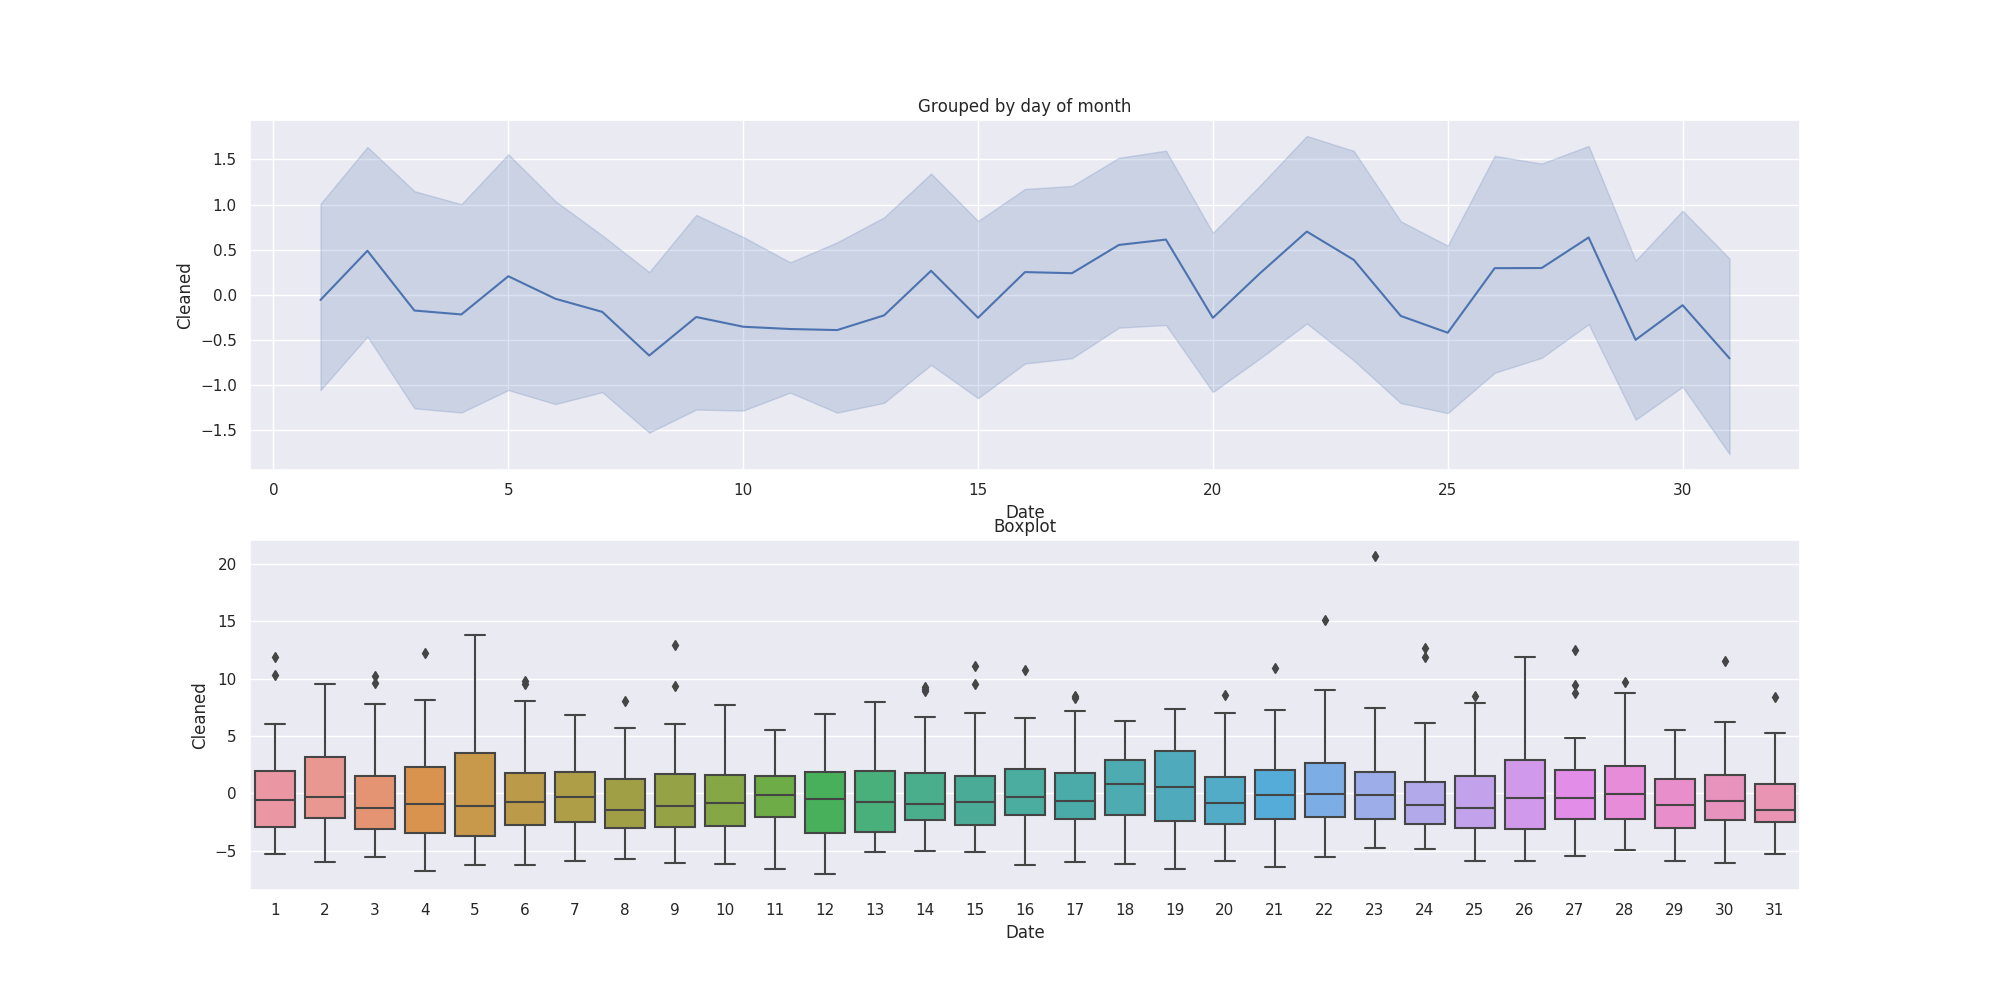
\includegraphics[width=0.7\textwidth]{plots/within_month.png}
  \caption{Retraso medio por d\'ia del mes}
  \label{fig:within_month}
\end{figure}

\begin{figure}[hbtp]
  \centering
  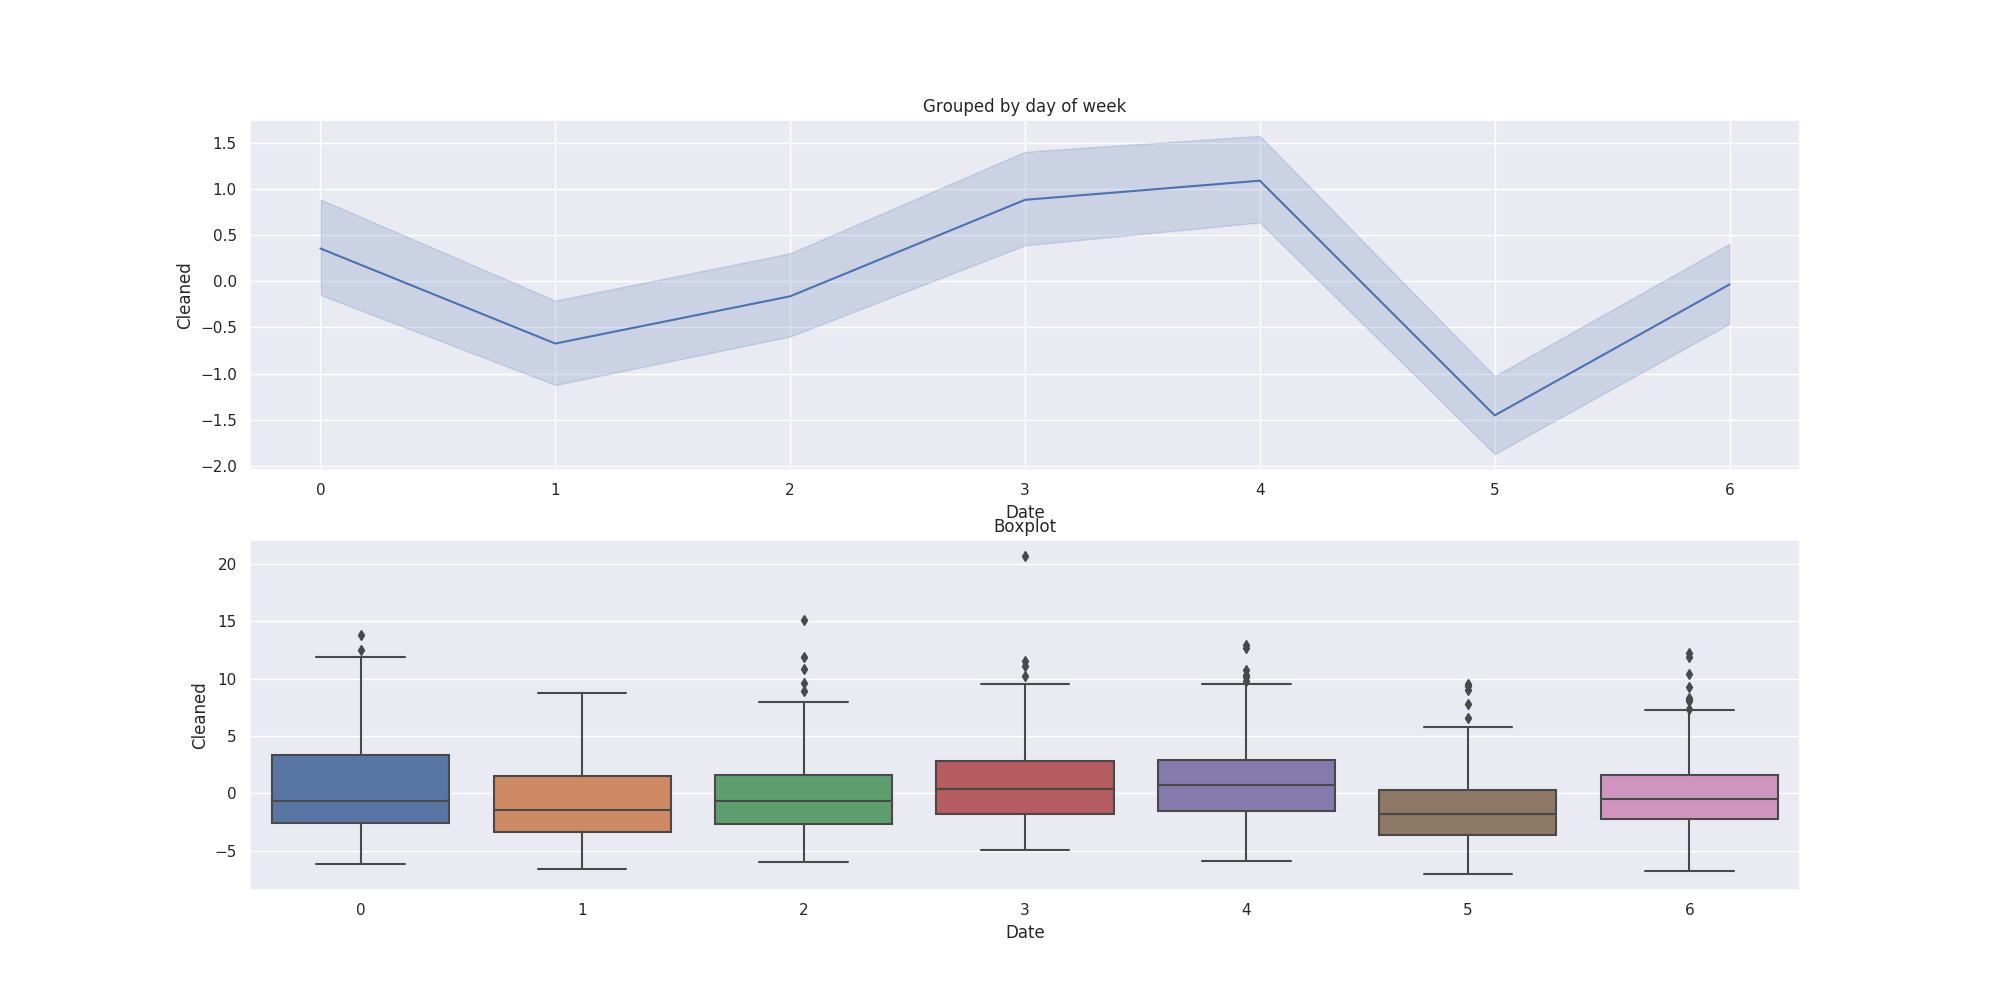
\includegraphics[width=0.7\textwidth]{plots/within_week.png}
  \caption{Retraso medio por d\'ia de la semana}
  \label{fig:within_week}
\end{figure}

Las figuras muestran un comportamiento peri\'odico de los retrasos. Es m\'as claro el de la figura \ref{fig:within_year}
que tiene elevaciones en los meses diciembre/enero y junio/julio, que es esperable pues son
meses de vacaciones. Tambi\'en se ve en la figura \ref{fig:within_week} un aumento en los d\'ias mi\'ercoles/jueves
y domingo/lunes. El comportamiento parece ser menos predecible para la figura \ref{fig:within_month}.

A modo de ejemplo, se muestran los m\'as altos scores
(explicados en la secci\'on \ref{subsec:scores}) del a\~no 2008
en las figuras \ref{fig:carrier_scores} y \ref{fig:airport_scores}.

\begin{figure}[hbtp]
  \centering
  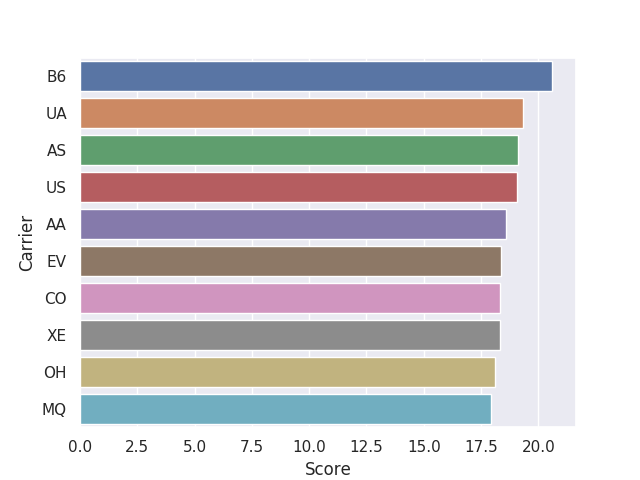
\includegraphics[width=0.7\textwidth]{plots/carrier_scores_2008.png}
  \caption{Carrier scores}
  \label{fig:carrier_scores}
\end{figure}

\begin{figure}[hbtp]
  \centering
  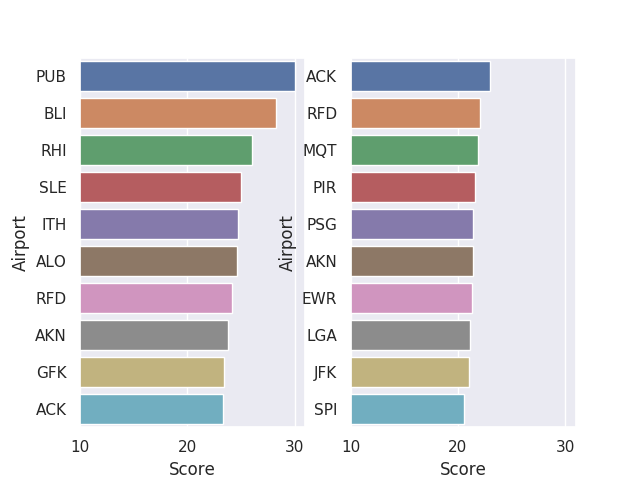
\includegraphics[width=\textwidth, height=3in]{plots/airport_scores_2008.png}
  \caption{Scores de aeropuertos (de origen y de destino)}
  \label{fig:airport_scores}
\end{figure}

